The system shall consist of four main elements: the sensor, the \gls{rpi}, \gls{coap} and the cloud platform.
The sensor will collect the data and pass this to the \gls{rpi}. The \gls{rpi} will then be responsible for manipulating
the data into a suitable format for transmission via \gls{coap}. The implementation of \gls{coap} will communicate with
the cloud platform. The cloud platform will store the data, allowing access to users.

\begin{figure}[H]
    \centering
    \makebox[1\textwidth]{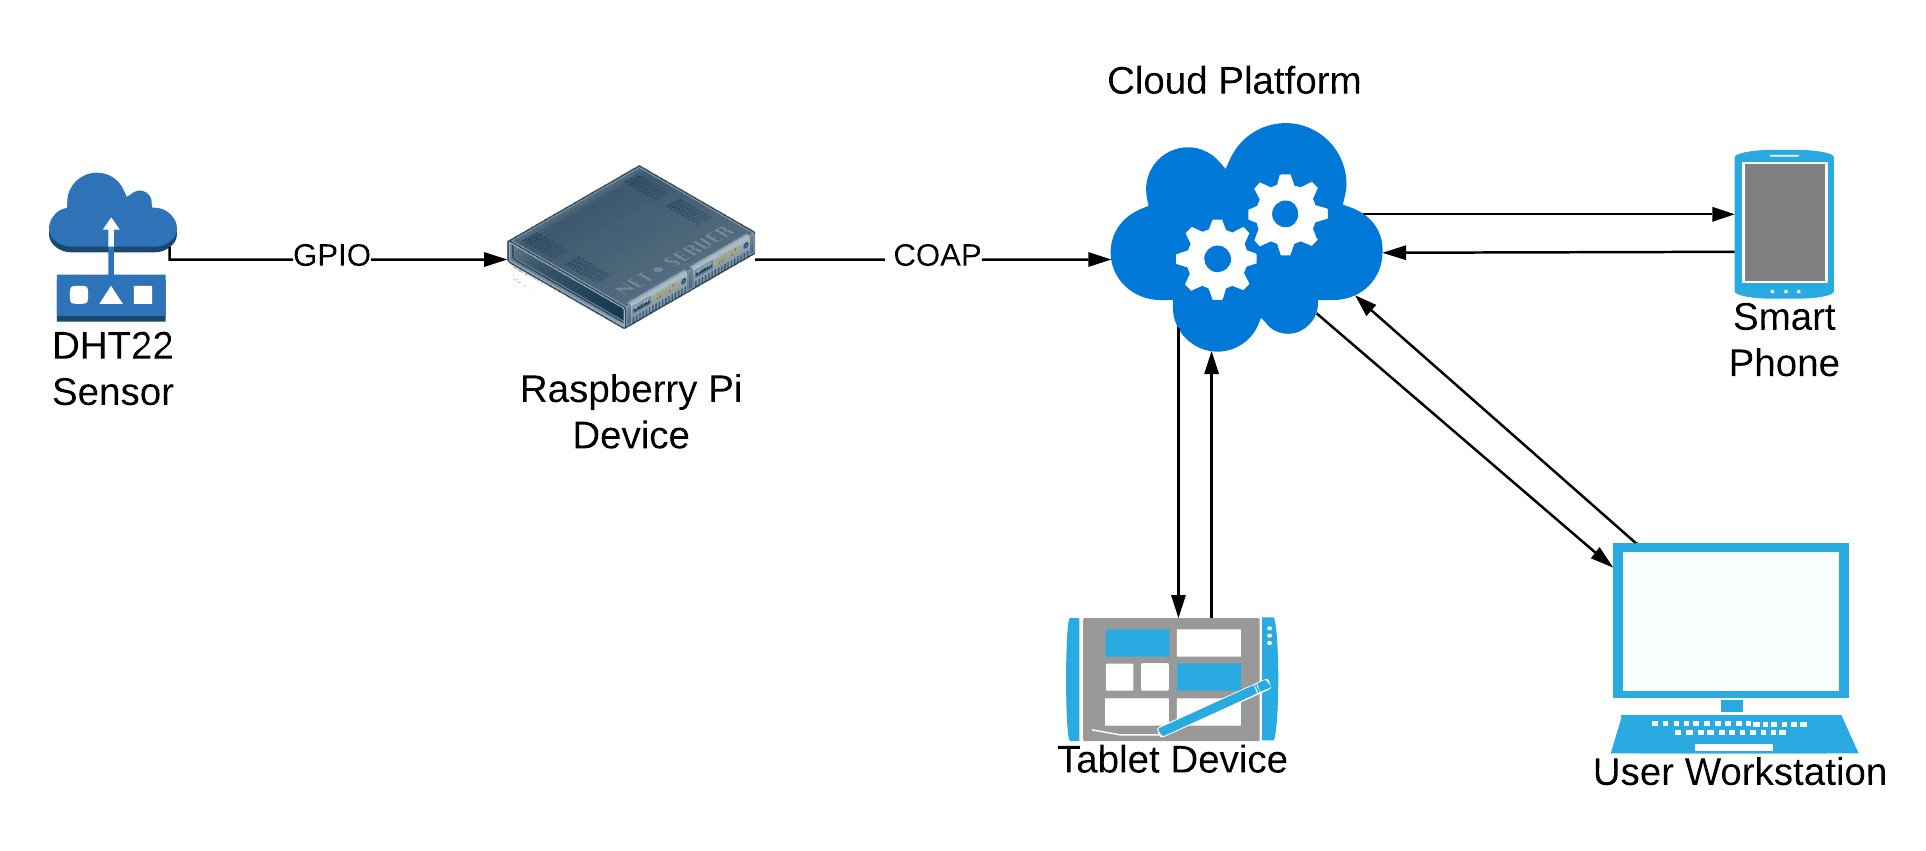
\includegraphics[width=1\textwidth]{assets/Project_Framework.png}}
    \caption{\label{fig:proj_framework} The project infrastructure.}
\end{figure}


The DHT22 sensor will connect to the \gls{rpi} using the \gls{rpi}'s on board \gls{gpio} ports as shown in \figref{fig:rpi_wiring}. 
Using the AdaFruit Python DHT library, a library that provides methods to interact with DHT sensors connected to the \gls{rpi}'s \gls{gpio} pins, 
and the CoAPthon library, a Python implementation of the \gls{coap} protocol, a Python script will create a \gls{coap} endpoint. This endpoint will expose 
the DHT methods for getting the latest data. When this endpoint receives a request the data will be current temperature and humidity will be
retrieved from the sensor. Once this data has been collected it will be formatted in to \gls{json} using Python. This formatted data will then
be the payload for the response. The cloud service will be responsible for displaying the data from the sensor and making the request to the 
\gls{rpi} to get up to date information. This process is shown in \figref{fig:data_flow}.


\begin{figure}[H]
    \centering
    \makebox[1\textwidth]{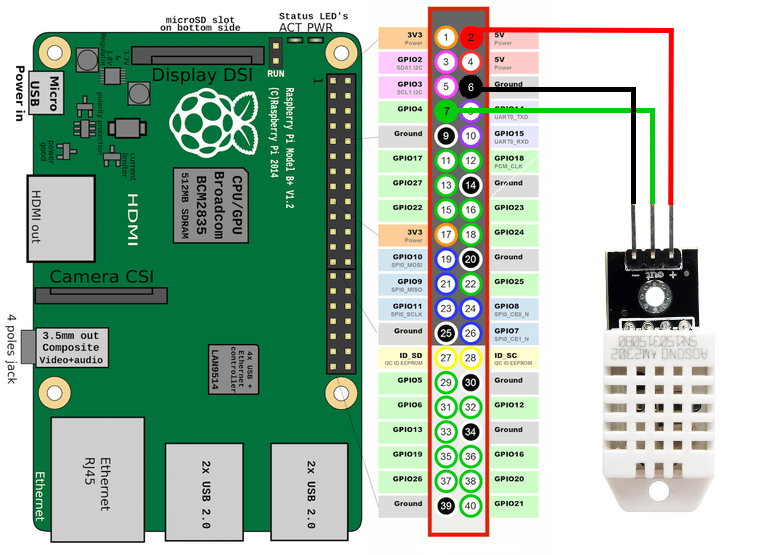
\includegraphics[width=1\textwidth]{assets/rpi_wiring.png}}
    \caption{\label{fig:rpi_wiring} Wiring diagram for connecting the sensor to the \gls{rpi}.}
\end{figure}

\begin{figure}[H]
    \centering
    \makebox[1\textwidth]{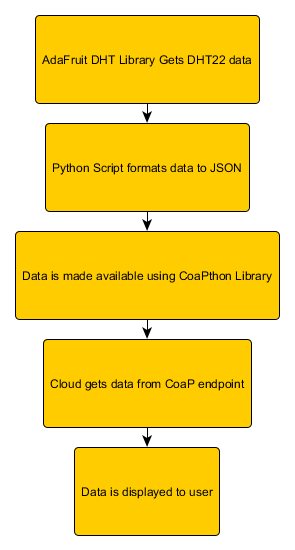
\includegraphics[width=0.5\textwidth]{assets/data_flow.png}}
    \caption{\label{fig:data_flow} Shows the flow of data from sensor to user.}
\end{figure}
